\chapter{Knapsack Problem}

\section{Descrizione del problema}

Il \textbf{Problema dello Zaino} (o \emph{Subset Sum}) è formalmente
definito come segue:

\begin{myblockquote}
  Ci sono $n$ oggetti $\{1, \ldots, n\}$, a ognuno viene assegnato un
  peso non negativo $w_i$ (per $i = 1, \ldots, n$ ) e viene dato anche
  un limite $W$ (capienza dello zaino).\\ L'obbiettivo è quello di
  selezionare un sottoinsieme $S$ degli oggetti tale che
  $\sum_{i \in S}w_i \leq W$ e che questa sommatoria abbia valore più
  grande possibile.
\end{myblockquote}

Questo problema è un caso specifico di un problema più generale
conosciuto come il Knapsack Problem, in cui l'unica differenza sta nel
valore da massimizzare, che per il Knapsack è un valore $v_i$ e non
più il peso.\\

Si potrebbe pensare di risolvere questi problemi con un algoritmo greedy
ma purtroppo non ne esiste uno in grado di trovare efficientemente la
soluzione ottima.\\

Un altro possibile approccio potrebbe essere quello di
ordinare gli oggetti in base al peso in ordine crescente o decrescente e
prenderli, tuttavia questo approccio fallisce per determinati casi (come
per l'insieme $\{W/2+1, W/2, W/2\}$ ordinato in senso decrescente) e
l'unica opzione sarà quella di provare con la programmazione dinamica.


\subsection{Goal}

Possiamo riassumere il goal di questa tipologia di problemi come segue:
\begin{myblockquote}
  Ci sono $n$ oggetti $\{1, \ldots, n\}$, a ognuno
  viene assegnato un peso non negativo $w_i$ (per $i = 1, \ldots, n$ )
  e ci viene dato anche un limite $W$.\\  L'obbiettivo è
  quello di selezionare un sottoinsieme $S$ degli oggetti tale che
  $\sum_{i \in S}w_i \leq W$ e che questa sommatoria abbia valore più
  grande possibile.
\end{myblockquote}


\section{Dynamic Version}

Come per tutti gli algoritmi dinamici dobbiamo cercare dei
\textbf{sotto-problemi} e possiamo utilizzare la stessa intuizione avuta
per il problema dello scheduling (scelta binaria in cui un oggetto viene
incluso nell'insieme o meno). Facendo tutti i calcoli di dovere,
otteniamo la seguente ricorsione:
\begin{myblockquote}
  \begin{itemize}
    \item se $W < w_i$ allora:
          $OPT(i, W) = OPT(i-1,W)$
    \item altrimenti:
          $OPT(i, W) = \max(OPT(i-1, W), w_i + OPT(i-1, W-w_i))$
  \end{itemize}
\end{myblockquote}

Nella prima parte analizziamo il caso in cui l'elemento che vogliamo
aggiungere va a superare il peso massimo residuo $W$, dunque viene
\textbf{scartato}.

Nella seconda parte andiamo ad analizzare se l'aggiunta o meno del
nuovo oggetto va a migliorare la soluzione (viene quindi
\textbf{selezionato}) di $OPT$ che è definita come:
$$
  OPT(i, w) = \max_{S} \sum_{j \in S} w_j
$$

Possiamo formalizzare il tutto con il seguente pseudo-codice:

\begin{lstlisting}[language=Python, mathescape=true]
for w = 0 to W 
	M[0, w] $\leftarrow$ 0
	
for j = 1 to n
	for w = 1 to W
		if(wj>W) 
			M[j,W] $\leftarrow$ M[j$-$1,W]
		
    else 
			M[j, W] $\leftarrow$ max { M [j $-$ 1, W], vj + M [j $-$ 1, W $-$ wj] }

return M[n,W]
\end{lstlisting}

\begin{figure}[H]
  \centering
  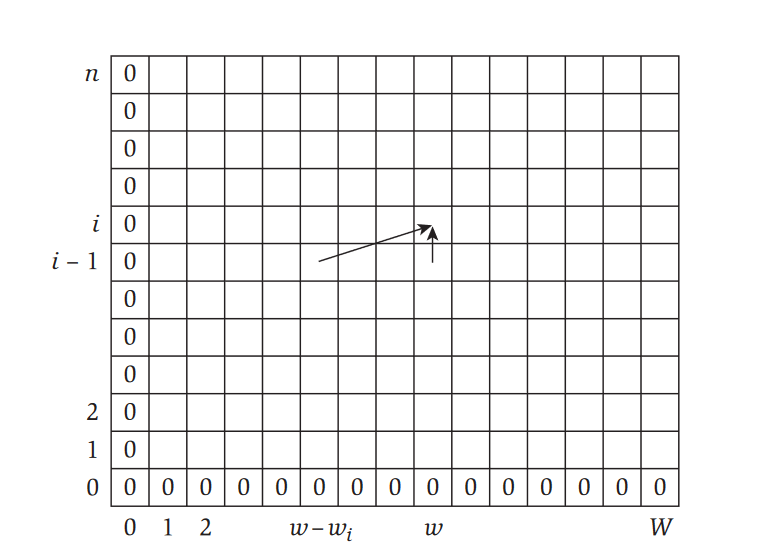
\includegraphics[width=\textwidth, keepaspectratio]{capitoli/programmazione_dinamica/imgs/knapsack_opt.png}
  \caption{La tabella bidimensionale dei valori di $OPT$.
    La colonna più a sinistra e l'ultima riga sono sempre 0. L'entry
    per $OPT(i, w)$ si calcola come indicato dalle frecce.}
\end{figure}


\subsection{Find Solution}

Dopo aver computato il valore ottimo, per trovare la soluzione completa
prendo come soluzione l'oggetto di inidce $i$ in $OPT(i, w)$ se e solo se
$M[i, w] > M[i-1, w]$,
poi se ho incluso $i$ nella soluzione mi sposto sotto di 1 ($j-1$) e a
sinistra di tante celle quanto è il peso dell'oggetto inserito, sennò non
mi muovo a sinistra e continuo solo scendendo di 1. Continuo questa
procedura fin quando non arrivo alla riga di indice 0. Tutto questo è
riassunto nel seguente pseudocodice.
\newpage
\begin{lstlisting}[language=Python, mathescape=true]
  // come invochi la funzione per far paretire la ricorsione
  // Find-Solution(n, W)
  function Find-Solution(j, w) {
    if (j == 0) {
      ritorna la soluzione
    }
  
    if (M[j, w] > M[j$-$1, w]) {
      includi j nella soluzione 
      Find-Solution(j$-$1, w$-$wj)
    }
  
    Find-Solution(j$-$1, w)
  }
\end{lstlisting}

\subsection{Costi}

\begin{center}
  \begin{tabular}{ |c|c|c| }
    \hline
    \textbf{Funzione} & \textbf{Costo in tempo} & \textbf{Costo in spazio} \\
    \hline
    Subset-Sum        & $\Theta(nW)$            & $\Theta(nW)$             \\
    \hline
    Find-Solution     & $O(n)$                  &                          \\
    \hline
  \end{tabular}
\end{center}

\begin{itemize}

  \item
        $O(1)$ per ogni elemento inserito nella tabella
  \item
        $\Theta(nW)$ elementi della tabella
\end{itemize}


\subsection{Osservazioni}

\begin{itemize}
  \item La particolarità di questo algoritmo è che avremmo 2 insiemi di sotto
        problemi diversi che devono essere risolti per ottenere la soluzione
        ottima. Questo fatto si riflette in come viene popolato l'array di
        memoization dei valori di $OPT$ che verranno salvati in un array
        bidimensionale (dimensione dell'input non polinomiale,
        pseudopolinomiale, perchè dipende da due variabili).

        \begin{figure}[H]
          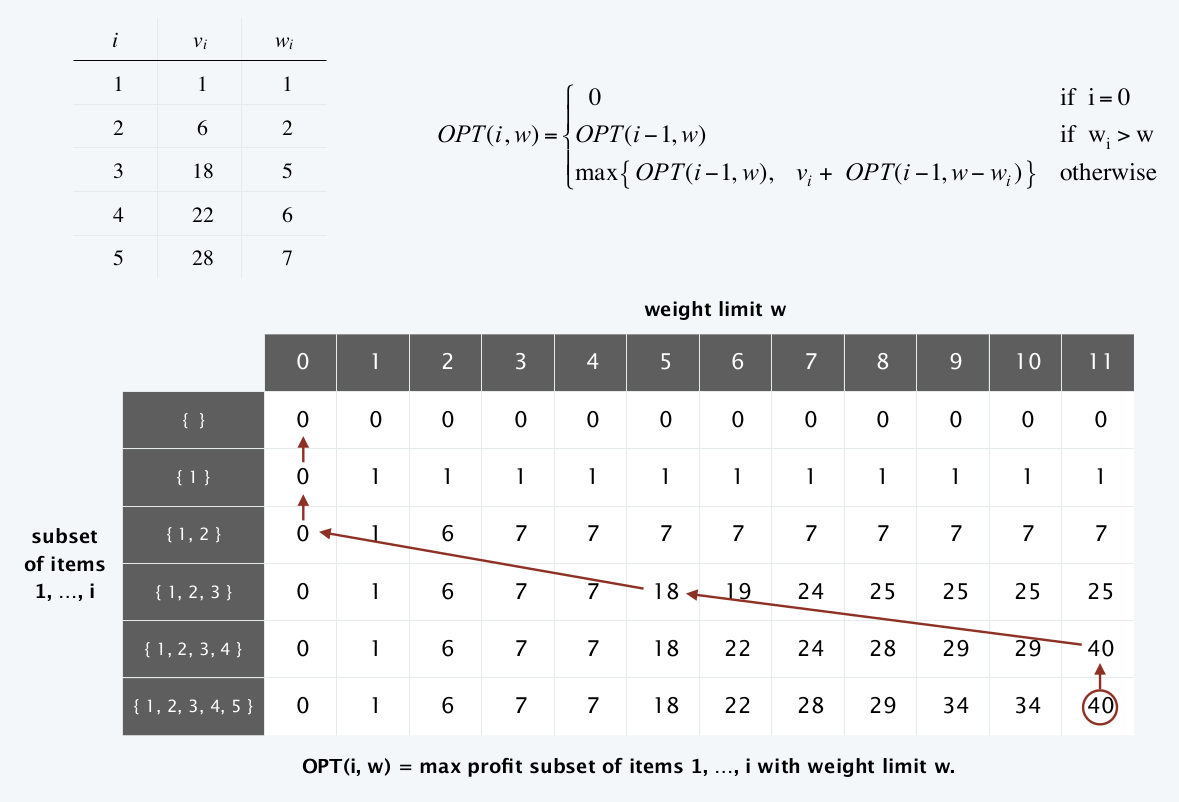
\includegraphics[width=13cm, keepaspectratio]{capitoli/programmazione_dinamica/imgs/zaino1.png}
          \centering
          \caption{In questa immagine si può vedere come è possibile ricostruire la soluzione
            salvata nell'array bidimensionale di memoization}
        \end{figure}

  \item A causa del costo computazionale $O(nW)$, questo algoritmo fa parte
        della famiglia degli algoritmi \emph{pseudo polinomiali}, ovvero
        algoritmi il cui costi dipende da una variabile di input che se
        piccola, lo mantiene basso e se grande lo fa esplodere. Ovvero, la
        versione del problema con decisione è \textbf{NP-Completo}.
  \item Per recuperare gli oggetti dall'array di Memoization la complessità in
        tempo è di $O(n)$.
  \item Questa implementazione funziona anche per il problema più generale del
        Knapsack, ci basterà solo cambiare la parte di ricorsione scrivendola
        come segue:\\
        \begin{myblockquote}
          \begin{itemize}
            \item se $W < w_i$ allora: $OPT(i, W) = OPT(i-1,W)$
            \item altrimenti: \linebreak $OPT(i, W) = \max(OPT(i-1, W), v_i + OPT(i-1, W-w_i))$
          \end{itemize}
        \end{myblockquote}

  \item Esiste un algoritmo che trova una soluzione in tempo polinomiale entro
        l'1\% di quella ottima.
\end{itemize}

\section{Riepilogo}

\begin{itemize}
  \item Scegliere gli oggetti da mettere nello zaino per massimizzare il
        valore, non superando il peso massimo.
  \item $OPT[i,w] = \max(v_i + OPT[i-1, w-w_i], OPT[i-1,w])$
  \item \textbf{Scelgo se prendere o meno l'oggetto} $i$
  \item Ho bisogno di una matrice $n \times W$ ($W$ è la capacità dello
        zaino). problema pseudopolinomiale perchè varia in base a $W$
        $\rightarrow$ \textbf{SPAZIO =} $O(nW)$
  \item Per riempire una cella devo solo controllare due valori
        $\rightarrow$ \textbf{TEMPO =} $O(nW)$
  \item In questo problema la matrice può essere costruita per righe o per
        colonne
  \item Per trovare $(i,w)$ leggo solo da una riga, per costrure la riga
        $i$ ho solo bisogno della riga $i-1$, la soluzione è in
        $S[n,W]$. Posso quindi trovare una soluzione utilizzando una matrice
        con sole due righe \textbf{SPAZIO =} $O(W)$ ma cosí non posso
        ricostruire la soluzione.
\end{itemize}
